\documentclass[preprint,12pt]{elsarticle}
\makeatletter
\def\ps@pprintTitle{%
	\let\@oddhead\@empty
	\let\@evenhead\@empty
	\def\@oddfoot{}%
	\let\@evenfoot\@oddfoot}
\makeatother
\usepackage[utf8]{inputenc}
\usepackage{graphicx}
\usepackage{url}
\usepackage{gensymb}
\usepackage{textcomp}
\usepackage{hyperref}
\usepackage{parskip}
\usepackage{commath}
\usepackage{float}
\usepackage{natbib}
\usepackage{doi}
\graphicspath{ {./images/} }
\usepackage{hyperref}
%
\makeatletter
\setlength{\@fptop}{0pt}
\makeatother
%
\usepackage{geometry}
\usepackage{amsmath}
\usepackage{amsthm}
\usepackage{amsfonts}
\usepackage{ upgreek }

\usepackage[export]{adjustbox}
\newtheorem{theorem}{Theorem}[section]
\newtheorem{corollary}{Corollary}[theorem]
\newtheorem{claim}{Claim}
\usepackage{subfigure}


\begin{document}

\begin{frontmatter}

\title{Logarithmic Spirals and Right-angled Triangles}

\author{Rahul Gohil}

\address{Student, B.E(Computer Engineering), Thadomal Shahani Engineering College, Mumbai, India\\Affiliated to University of Mumbai}
\ead{rahul.gohil@thadomal.org}
\begin{abstract}
This article presents some recurrent functions which we can use to make Right-angled Triangles and through their special arrangement we can obtain logarithmic spirals, and their discrete form. The recurrent functions are obtained through recurrence relations which can be expressed as a linear combination of fibonacci numbers.  
\end{abstract}

\begin{keyword}
Logarithmic Spirals \sep Kepler Triangles\sep Discrete Logarithmic Spirals \sep Recurrent Functions 
\end{keyword}

\end{frontmatter}

\section{Introduction}
G. Anatriello, et al\cite{paper1} discussed about continue triangles and how they discretize a logarithmic spiral by polygon chains and obtained different discrete spirals known as $(r, k)$-male spirals which discretize well known logarithmic spirals. Here we give a different approach for discretization of logarithmic spiral using right-angled triangles.
 
\subsection{Recurrence relations which are linear combination of fibonacci numbers}
\label{recurr}
Let's take the Fibonacci sequence, $f'(n) = f'(n - 1) + f'(n - 2)$, where $f'(0) = 0$ \& $f'(1) = 1$.\\
It's easy to see that for $A  = \begin{bmatrix}1 & 1 \\ 1 & 0 \end{bmatrix}$ $$A^n = \begin{bmatrix}f'(n + 1) & f'(n) \\ f'(n) & f'(n - 1)\end{bmatrix}$$
Let's take a sequence of recurrence relations $f_{a,b,c}$ such that\\ $f_{a,b,c}(n)^a = f_{a,b,c}(n - b)^a+f_{a,b,c}(n - c)^a$, where $\{f_{a,b,c}(0), f_{a,b,c}(1), \ldots, f_{a,b,c}(c - 1)\}$ is given, $a > 0$, $c > b > 0$ are integers \\
We can define this sequence in matrix form as
\begin{align*}
\begin{bmatrix}f_{a,b,c}(n)^a \\f_{a,b,c}(n - b)^a\end{bmatrix} 
&=
\begin{bmatrix}1 & 1\\1 & 0\end{bmatrix}
\begin{bmatrix}f_{a,b,c}(n - b)^a\\f_{a,b,c}(n - c)^a\end{bmatrix}
\end{align*}
Let $h$ be a positive integer such that the following relation holds.
\begin{align*}
\begin{bmatrix}f_{a,b,c}(n)^a \\f_{a,b,c}(n - b)^a\end{bmatrix}
&=
\begin{bmatrix}1 & 1\\1 & 0\end{bmatrix}^h
\begin{bmatrix}f_{a,b,c}(n - hb)^a\\f_{a,b,c}(n-(h-1)b - c)^a\end{bmatrix}\\
\text{Therefore}\\
\begin{bmatrix}f_{a,b,c}(n)^a \\f_{a,b,c}(n - b)^a\end{bmatrix}
&=
\begin{bmatrix}f'(h+1) & f'(h)\\f'(h) & f'(h-1)\end{bmatrix}
\begin{bmatrix}f_{a,b,c}(n - hb)^a\\f_{a,b,c}(n-(h-1)b - c)^a\end{bmatrix}
\stepcounter{equation}\tag{\theequation}\label{myeq1}\\
\end{align*}
We get that $f_{a,b,c}(n)^a = f'(h+1)f_{a,b,c}(n-hb)^a + f'(h)f_{a,b,c}(n-(h-1)b-c)^a$
$$f_{a,b,c}(n-b)^a+f_{a,b,c}(n-c)^a=f'(h+1)f_{a,b,c}(n-hb)^a +f'(h)f_{a,b,c}(n-(h-1)b-c)^a$$
Substituting $f_{a,b,c}(n-b) = f'(h)f_{a,b,c}(n-hb)^a+f'(h-1)f_{a,b,c}(n-(h-1)b-c)^a$
\begin{multline*}
	f'(h)f_{a,b,c}(n-hb)^a+f'(h-1)f_{a,b,c}(n-(h-1)b-c)^a + f_{a,b,c}(n-c)^a =\\f'(h+1)f_{a,b,c}(n-hb)^a +f'(h)f_{a,b,c}(n-(h-1)b-c)^a\\\\
	f_{a,b,c}(n-c)^a = f'(h+1)f_{a,b,c}(n-hb)^a +f'(h)f_{a,b,c}(n-(h-1)b-c)^a \\-f'(h)f_{a,b,c}(n-hb)^a-f'(h-1)f_{a,b,c}(n-(h-1)b-c)^a\\\\
	f_{a,b,c}(n-c)^a = f'(h-1)f_{a,b,c}(n-hb)^a+f'(h-2)f_{a,b,c}(n-(h-1)b-c)^a\\
\end{multline*}
Let's look at the equation of $f_{a,b,c}(n-c)^a$ for 2 values of $h$, $k$ and $k+1$ and equate.
\begin{multline*}
	f'(k-1)f_{a,b,c}(n-kb)^a+f'(k-2)f_{a,b,c}(n-(k-1)b-c)^a =\\ f'(k)f_{a,b,c}(n-(k+1)b)^a+f'(k-1)f_{a,b,c}(n-kb-c)^a\\\\
	f'(k-1)f_{a,b,c}(n-kb)^a+f'(k-2)f_{a,b,c}(n-(k-1)b-c)^a =
	f'(k-1)f_{a,b,c}(n-(k+1)b)^a\\+f'(k-2)f_{a,b,c}(n-(k+1)b)^a +f'(k-1)f_{a,b,c}(n-kb-c)^a
\end{multline*}
Since $f_{a,b,c}(n-kb)^a = f_{a,b,c}(n-(k+1)b)^a+f_{a,b,c}(n-kb-c)^a$
\begin{multline*}
	f'(k-1)f_{a,b,c}(n-kb)^a+f'(k-2)f_{a,b,c}(n-(k-1)b-c)^a =\\ f'(k-1)f_{a,b,c}(n-kb)^a+f'(k-2)f_{a,b,c}(n-(k+1)b)^a
\end{multline*}
$$f'(k-2)f_{a,b,c}(n-(k-1)b-c)^a = f'(k-2)f_{a,b,c}(n-(k+1)b)^a$$
Therefore we can say that $$n-(k-1)b -c = n-(k+1)b$$
$$n-kb+b-c=n-kb-b$$
$$c = 2b$$
Therefore $$f_{a,b,c}(n)^a = f_{a,b}(n)^a = f_{a,b}(n-b)^a+f_{a,b}(n-2b)^a$$ under the relation mentioned at ~\eqref{myeq1}.\\
A. Fiorenza et al\cite{paper2} discussed about the limit of consecutive terms of generalized homogeneous recurrences and proved that the limit exists. 
Now, if $0 \leq n-(h+1)b < b$, the integer solution of $h$ is $h = \left\lfloor\dfrac{n}{b}\right\rfloor - 1$.
\begin{align*}
	\begin{bmatrix}f_{a,b}(n)^a \\f_{a,b}(n - b)^a\end{bmatrix}
	&=
	\begin{bmatrix}1 & 1\\1 & 0\end{bmatrix}^h
	\begin{bmatrix}f_{a,b}(n - hb)^a\\f_{a,b}(n-(h+1)b)^a\end{bmatrix}\\
	\begin{bmatrix}f_{a,b}(n)^a \\f_{a,b}(n - b)^a\end{bmatrix}
	&=
	\begin{bmatrix}f'(h+1) & f'(h)\\f'(h) & f'(h-1)\end{bmatrix}
	\begin{bmatrix}f_{a,b}(n - hb)^a\\f_{a,b}(n-(h+1)b)^a\end{bmatrix}\\
	\text{Let $\lambda_{n}=\left\lfloor\dfrac{n}{b}\right\rfloor$, $h = \lambda_{n} - 1$}\\
	\begin{bmatrix}f_{a,b}(n)^a \\f_{a,b}(n - b)^a\end{bmatrix}
	&=
	\begin{bmatrix}f'(\lambda_n) & f'(\lambda_{n}-1)\\f'(\lambda_n-1) & f'(\lambda_n-2)\end{bmatrix}
	\begin{bmatrix}f_{a,b}(n - hb)^a\\f_{a,b}(n-(h+1)b)^a\end{bmatrix}
\end{align*}
Let $m_n = n \mod b = n - \lambda_nb$\\
$$\begin{bmatrix}f_{a,b}(n)^a \\f_{a,b}(n - b)^a\end{bmatrix}
=
\begin{bmatrix}f'(\lambda_n) & f'(\lambda_{n}-1)\\f'(\lambda_n-1) & f'(\lambda_n-2)\end{bmatrix}
\begin{bmatrix}f_{a,b}(b+m_n)^a\\f_{a,b}(m_n)^a\end{bmatrix}$$
Therefore $$f_{a,b}(n)^a = f'(\lambda_n)f_{a,b}(b+m_n)^a+f'(\lambda_n-1)f_{a,b}(m_n)^a$$
\begin{theorem}
	\label{lim-cons}
	$$\lim_{n \to \infty} \dfrac{f_{a,b}(n + p)}{f_{a,b}(n + q)} = \left(c_{p',q'}\varphi^{d_{p',q'}}\right)^{1/a}$$\\
	such that $c_{p',q'} = \dfrac{\varphi f_{a,b}(b+m_{p'})^a + f_{a,b}(m_{p'})^a}{\varphi f_{a,b}(b+m_{q'})^a + f_{a,b}(m_{q'})^a}$\\
	\begin{equation*}
		d_{p', q'} = \lambda_{p'} - \lambda_{q'} = \begin{cases}
		h - k & h_1 = k_1 = 0 \hspace{2mm}or\hspace{2mm} \{h_1,k_1\} \in \mathbf{Z_b} - \{0\}\\
		h - k - 1 & h_1 = 0, k_1 \in \mathbf{Z_b} - \{0\} \hspace{2mm}or\hspace{2mm} h_1 \in \mathbf{Z_b} - \{0\}, k_1 = 0
		\end{cases}
	\end{equation*}
	where $p' = n + p = hb - h_1 \mid hb \geq p' > (h-1)b, h_1\in\mathbf{Z_b}$\\
	and $q' = n + q = kb - k_1 \mid kb \geq q' > (k-1)b, k_1\in\mathbf{Z_b}$
\end{theorem}
\begin{proof}
	\begin{align*}
		\dfrac{f_{a,b}(n+p)}{f_{a,b}(n+q)} &= \left(\dfrac{f'(\lambda_{p'})f_{a,b}(b+m_{p'})^a + f'(\lambda_{p'}-1)f_{a,b}(m_{p'})^a}{f'(\lambda_{q'})f_{a,b}(b+m_{q'})^a + f'(\lambda_{q'}-1)f_{a,b}(m_{q'})^a}\right)^{1/a}\\\\
		&= \left(\dfrac{f'(\lambda_{p'}-1)\left(\dfrac{f'(\lambda_{p'})}{f'(\lambda_{p'}-1)}f_{a,b}(b+m_{p'})^a + f_{a,b}(m_{p'})^a\right)}{f'(\lambda_{q'}-1)\left(\dfrac{f'(\lambda_{q'})}{f'(\lambda_{q'}-1)}f_{a,b}(b+m_{q'})^a + f_{a,b}(m_{q'})^a\right)}\right)^{1/a}\\\\
		\lim_{n \to \infty}\dfrac{f_{a,b}(n+p)}{f_{a,b}(n+q)} &=
		\left(\dfrac{f'(\lambda_{p'}-1)\left(\varphi f_{a,b}(b+m_{p'})^a + f_{a,b}(m_{p'})^a\right)}{f'(\lambda_{q'}-1)\left(\varphi f_{a,b}(b+m_{q'})^a + f_{a,b}(m_{q'})^a\right)}\right)^{1/a}
	\end{align*}
		Let $c_{p',q'} = \dfrac{\varphi f_{a,b}(b+m_{p'})^a + f_{a,b}(m_{p'})^a}{\varphi f_{a,b}(b+m_{q'})^a + f_{a,b}(m_{q'})^a}$\\
	$\dfrac{f'(\lambda_{p'} - 1)}{f'(\lambda_{q'} - 1)} = \dfrac{\varphi^{\lambda_{p'} - 1}\sqrt{5}}{\varphi^{\lambda_{q'} - 1}\sqrt{5}} = \dfrac{\varphi^{\lambda_{p'}}}{\varphi^{\lambda_{q'}}}$\\\\
	Let $d_{p', q'} = \lambda_{p'} - \lambda_{q'}$\\
	$\lambda_{p'} = \left\lfloor\dfrac{n + p}{b}\right\rfloor$, $\lambda_{q'} = \left\lfloor\dfrac{n + q}{b}\right\rfloor$, we can choose such $h$ and $k$ that,\\
	$\left\lfloor\dfrac{n + p}{b}\right\rfloor = hb - h_1$, $\left\lfloor\dfrac{n + q}{b}\right\rfloor = kb - k_1$,\\where $p'= n + p = hb - h_1 \mid hb \geq p' > (h-1)b, h_1\in\mathbf{Z_b}$\\
	and $q' = n + q = kb - k_1 \mid kb \geq q' > (k-1)b, k_1\in\mathbf{Z_b}$\\\\
	\begin{equation*}
		\left\lfloor\dfrac{n + p}{b}\right\rfloor = \begin{cases}
		h & h_1 = 0\\
		h - 1 & h_1 \in \mathbf{Z_b} - \{0\}
		\end{cases}
	\end{equation*}
	\begin{equation*}
	\left\lfloor\dfrac{n + q}{b}\right\rfloor = \begin{cases}
	k & k_1 = 0\\
	k - 1 & k_1 \in \mathbf{Z_b} - \{0\}
	\end{cases}
	\end{equation*}
	Therefore,\\
	\begin{equation*}
	\left\lfloor\dfrac{n + p}{b}\right\rfloor -\left\lfloor\dfrac{n + q}{b}\right\rfloor  = \begin{cases}
	h - k & h_1 = 0, k_1 = 0 \hspace{2mm}or\hspace{2mm}\{h_1, k_1\} \in \mathbf{Z_b} - \{0\}\\
	h - k - 1 & h_1 \in \mathbf{Z_b} - \{0\}, k_1 = 0\hspace{2mm}or\hspace{2mm} h_1= 0, k_1 \in \mathbf{Z_b} - \{0\}
	\end{cases}
	\end{equation*}
	
	Therefore,\\
	$$\lim_{n \to \infty} \dfrac{f_{a,b}(n + p)}{f_{a,b}(n + q)} = \left(c_{p',q'}\varphi^{d_{p',q'}}\right)^{1/a}$$
\end{proof}
\subsection{Geometric Interpretation}
\label{geo}
Let $(x_1, y_1)$ be any point on the 2D Plane.Let $(f_{a,b}(0) + x_1, y_1)$ and $(f_{a,b}(0) + x_1, f_{a,b}(1) + y_1)$ be points on the plane, by connecting them we get the triangle.
Let $I_0 = (x_1, y_1)$ and $I_1 = (f_{a,b}(0) + x_1, y_1)$, we define a function $P$ which is point on the 2D Plane.\\
Let $P(0) = (f_{a,b}(0) + x_1, f_{a,b}(1) + y_1)$, the $P$ function has 2 class variables(a class variable is used to denote a variable associated with the object of that class in programming languages), namely $x$ and $y$, which denote the x co-ordinate and y co-ordinate of that point respectively.\\
We define $P(n)$ as
\begin{equation*}
P(n) = \begin{cases}
(P(n - 1).x - f_{a,b}(n + 1), P(n - 1).y) & n \equiv 1\mod 4\\
(P(n - 1).x, P(n - 1).y - f_{a,b}(n + 1)) & n \equiv 2\mod 4\\
(P(n - 1).x + f_{a,b}(n + 1), P(n - 1).y) & n \equiv 3\mod 4\\
(P(n - 1).x, P(n - 1).y + f_{a,b}(n + 1)) & n \equiv 0\mod 4
\end{cases}
\end{equation*}
We define a function $L$ which is a line on the 2D Plane.\\
Let $L(0) = (I_0, P(0))$, this means that $L(0)$ is a line between points $I_0$ and $P(0)$, $L(1) = (I_1, P(1))$. $L$ function has 5 class variables, namely $point1$, $point2$, $slope$, $constant$, $length$ denoting the first point in the tuple, the second point in the tuple, slope of the line, the constant associated with it and the length of the line respectively.\\
We define $L(n)$ as $$L(n) = (L(n - 2).point2, P(n))$$ 
Essentially $L(n)$ is the hypotenuse of the nth triangle.
We also define a function $L'$ which describes base and height of a triangle which has same class variables as $L$.
Let $L'(0) = (I_0, I_1)$ and $L'(1) = (I_1, P(0))$.
$$L'(n) = (L'(n - 1).point2, P(n - 1))$$
Let's also define a function for a triangle $T$, $T(0) = (L'(0), L'(1), L(0))$. $T$ function has 3 class variables $line1$, $line2$ and $line3$, denoting base, height and hypotenuse respectively.
$$T(n) = (T(n - 1).line2, L'(n + 1), L(n))$$
For each $n$, $L'(n)$ is the base, $L'(n + 1)$ is the height and $L(n)$ is the hypotenuse of triangle $T(n)$.\\
Through out this paper, we are going to assume $n$ being an integer such that $n \equiv 0\mod4$
\begin{theorem}
	\label{lim-P}
	$$\lim_{n \to \infty} P(n).x - x_1 = \varrho_{a,b}f_{a,b}(n - 2b)$$
	where $\varrho_{a,b} = \dfrac{\varphi^{2/a}}{\varphi^{2/a} - (-1)^b}\displaystyle\sum_{i = 0}^{b - 1}(-1)^i (c_{2i', 2b'}\varphi^{\lambda_{2i'}-\lambda_{n}+2})^{1/a}$
\end{theorem}
\begin{proof}
	$P(n).x$ can alternatively be defined as $$P(n).x = x_1 + \sum_{i = 0}^{n / 2}(-1)^i f_{a,b}(n-2i)$$.
	$$P(n).x - x_1 = \sum_{i = 0}^{n / 2}(-1)^i f_{a,b}(n-2i)$$
	Let $g(n) = \dfrac{P(n).x - x_1}{f_{a,b}(n - 2b)}$
	\begin{align*}
	g(n) &= \dfrac{\displaystyle\sum_{i = 0}^{n / 2}(-1)^i f(n-2i)}{f_{a,b}(n - 2b)}\\
	&= \sum_{i = 0}^{n / 2}\dfrac{(-1)^i f(n-2i)}{f_{a,b}(n - 2b)}\\
	\lim_{n \to \infty}g(n) &= \lim_{n \to \infty}\sum_{i = 0}^{n / 2}(-1)^i \dfrac{f(n-2i)}{f_{a,b}(n - 2b)}\\
	\text{Using \ref{lim-cons}}\\
	\lim_{n \to \infty}g(n) &= \lim_{n \to \infty}\sum_{i = 0}^{n / 2}(-1)^i (c_{2i',2b'}\varphi^{d_{2i',2b'}})^{1/a}
	\end{align*}
	Let $S(n) = \displaystyle\sum_{i = 0}^{n/2}(-1)^i (c_{2i',2b'}\varphi^{d_{2i',2b'}})^{1/a}$\\
	$d_{2i',2b'} = \lambda_{2i'}-\lambda_{2b'}=\lambda_{2i'}-\left\lfloor\dfrac{n-2b}{b}\right\rfloor = \lambda_{2i'}- \left\lfloor\dfrac{n}{b}\right\rfloor + 2 = \lambda_{2i'}-\lambda_{n}+2$\\
	$S(n) = \displaystyle\sum_{i = 0}^{n/2}(-1)^i (c_{2i',2b'}\varphi^{\lambda_{2i'}-\lambda_{n}+2})^{1/a}$\\
	$S(n)$ can be visualized as,\\
	\begin{align*}
		S(n) &= (-1)^0(c_{0',2b'}\varphi^{\lambda_{0'}-\lambda_{n}+2})^{1/a}+(-1)^{b}(c_{2b',2b'}\varphi^{\lambda_{2b'}-\lambda_{n}+2})^{1/a}+(-1)^{2b}(c_{2(2b)',2b'}\varphi^{\lambda_{2(2b)'}-\lambda_{n}+2})^{1/a}+\ldots\\\\
		&+(-1)^1(c_{2',2b'}\varphi^{\lambda_{2'}-\lambda_{n}+2})^{1/a}+(-1)^{b+1}(c_{2(b+1)',2b'}\varphi^{\lambda_{2(b+1)'}-\lambda_{n}+2})^{1/a}+\ldots\\\\
		&+\vdots\\
		&+(-1)^{b-1}(c_{2(b-1)',2b'}\varphi^{\lambda_{2(b-1)'}-\lambda_{n}+2})^{1/a}+(-1)^{2b-1}(c_{2(2b-1)',2b'}\varphi^{\lambda_{2(2b-1)'}-\lambda_{n}+2})^{1/a}+\ldots
	\end{align*}  
	\clearpage
	So, it is split into $b$ rows and $\lambda_{n/2} + 1$ columns, the last column contains $m_{n/2}$ terms and $b - m_{n/2}$ zeros. Each row represent a geometric series, let's see the common ratio for each row.\\
	For the first row,
	\begin{align*}
		\dfrac{(-1)^{b}(c_{b',2b'}\varphi^{\lambda_{b'}-\lambda_{n}+2})^{1/a}}{(-1)^0(c_{0',2b'}\varphi^{\lambda_{0'}-\lambda_{n}+2})^{1/a}} &= (-1)^b\left(\varphi^{\lambda_{2b'}-\lambda_{n}+2-\lambda_{0'}+\lambda_{n}-2}\right)^{1/a}\\
		&= (-1)^b\left(\varphi^{\lambda_{2b'}-\lambda_{0'}}\right)^{1/a}\\
		&= (-1)^b\left(\varphi^{\lambda_{n}-2-\lambda_{n}}\right)^{1/a}\\
		&=(-1)^b \varphi^{-2/a}
	\end{align*}
	For the second row,
	\begin{align*}
		\dfrac{(-1)^{b+1}(c_{2(b+1)',2b'}\varphi^{\lambda_{2(b+1)'}-\lambda_{n}+2})^{1/a}}{(-1)^{1}(c_{2',2b'}\varphi^{\lambda_{2'}-\lambda_{n}+2})^{1/a}} &= (-1)^b\left(\varphi^{\lambda_{2(b+1)'}-\lambda_{n}+2-\lambda_{2'}+\lambda_{n}-2}\right)^{1/a}\\
		&= (-1)^b\left(\varphi^{\lambda_{2(b+1)'}-\lambda_{2'}}\right)^{1/a}\\
		&= (-1)^b\left(\varphi^{\lambda_{2'}-2-\lambda_{2'}}\right)^{1/a}\\
		&=(-1)^b \varphi^{-2/a}
	\end{align*}
	For the $b$th row,
	\begin{align*}
	\dfrac{(-1)^{2b-1}(c_{2(2b-1)',2b'}\varphi^{\lambda_{2(2b-1)'}-\lambda_{n}+2})^{1/a}}{(-1)^{b-1}(c_{2(b-1)',2b'}\varphi^{\lambda_{2(b-1)'}-\lambda_{n}+2})^{1/a}} &= (-1)^b\left(\varphi^{\lambda_{2(2b-1)'}-\lambda_{n}+2-\lambda_{2(b-1)'}+\lambda_{n}-2}\right)^{1/a}\\
	&= (-1)^b\left(\varphi^{\lambda_{2(2b-1)'}-\lambda_{2(b-1)'}}\right)^{1/a}
	\end{align*}
	\begin{align*}
		\lambda_{2(2b-1)'}-\lambda_{2(b-1)'} &= \left\lfloor\dfrac{n-4b+2}{b}\right\rfloor-\left\lfloor\dfrac{n-2b+2}{b}\right\rfloor\\&=\left\lfloor\dfrac{n+2}{b}\right\rfloor-4-\left\lfloor\dfrac{n+2}{b}\right\rfloor+2\\ &= -2
	\end{align*}
	So, the common ratio for $b$th row $=(-1)^b \varphi^{-2/a}$\\
	Therefore $S(n)$ can be reduced to
	\begin{align*}
		S(n) &=  (-1)^0(c_{0',2b'}\varphi^{\lambda_{0'}-\lambda_{n}+2})^{1/a}\left(\dfrac{1 - ((-1)^b\varphi^{-2/a})^{\lambda_{n/2}+1}}{1-(-1)^b\varphi^{-2/a}}\right)\\\\
		&+(-1)^1(c_{2',2b'}\varphi^{\lambda_{2'}-\lambda_{n}+2})^{1/a}\left(\dfrac{1 - ((-1)^b\varphi^{-2/a})^{\lambda_{n/2}+1}}{1-(-1)^b\varphi^{-2/a}}\right)\\\\
		&+\vdots\\\\
		&+(-1)^{b-1}(c_{2(b-1)',2b'}\varphi^{\lambda_{2(b-1)'}-\lambda_{n}+2})^{1/a}\left(\dfrac{1 - ((-1)^b\varphi^{-2/a})^{\lambda_{n/2}+1}}{1-(-1)^b\varphi^{-2/a}}\right)
	\end{align*}
	\begin{align*}
		S(n) &= \left(\dfrac{1 - ((-1)^b\varphi^{-2/a})^{\lambda_{n/2}+1}}{1-(-1)^b\varphi^{-2/a}}\right)\displaystyle\sum_{i = 0}^{b-1}(-1)^i\left(c_{2i',2b'}\varphi^{\lambda_{2i'}-\lambda_{n}+2}\right)^{1/a}\\
		\lim_{n \to \infty}S(n) &= \left(\dfrac{1}{1-(-1)^b\varphi^{-2/a}}\right)\displaystyle\sum_{i = 0}^{b-1}(-1)^i\left(c_{2i',2b'}\varphi^{\lambda_{2i'}-\lambda_{n}+2}\right)^{1/a}\\
		\lim_{n \to \infty}S(n) &= \left(\dfrac{\varphi^{2/a}}{\varphi^{2/a}-(-1)^b}\right)\displaystyle\sum_{i = 0}^{b-1}(-1)^i\left(c_{2i',2b'}\varphi^{\lambda_{2i'}-\lambda_{n}+2}\right)^{1/a}\\
		\lim_{n \to \infty}S(n) &= \varrho_{a,b}\\
		\lim_{n \to \infty}g(n) &= \varrho_{a,b}
	\end{align*}
	$$
	\lim_{n \to \infty}\dfrac{P(n).x - x_1}{f_{a,b}(n - 2b)} = \varrho_{a,b}$$
	Therefore,
	$$\lim_{n \to \infty} P(n).x - x_1 = \varrho_{a,b}f_{a,b}(n - 2b)$$
\end{proof}
Similarly we can prove that,
\begin{align*}
&\lim_{n \to \infty} P(n).y -y_1 = \varrho_{a,b}f_{a,b}(n-2b+1)\\
&\lim_{n \to \infty} P(n+1).x -x_1 = -\varrho_{a,b}f_{a,b}(n-2b+2)
\end{align*}
\section{Some Properties}
Here, we will focus on $b =1$,\\

	1. As $n \to \infty$, angle between $L(n)$ and $L(n+1)$ tends $\to 90^\circ$

\begin{proof}
	Let $A(n)$ be angle between $L(n)$ and $L(n+1)$
	$$A(n) = \tan^{-1}\left({\abs{\dfrac{L(n+1).slope-L(n).slope}{1+(L(n+1).slope \cdot L(n).slope)}}}\right)$$
	Let $1 + (L(n+1).slope \cdot L(n).slope) = s$\\
	$L(n+1) = (P(n-1), P(n+1))$ and $L(n) = (P(n-2), P(n))$
	\begin{align*}
	L(n+1).slope &= \dfrac{s - 1}{L(n).slope}\\
	\dfrac{P(n+1).y - P(n-1).y}{P(n+1).x - P(n-1).x} &= \dfrac{(s-1)(P(n).x-P(n-2).x)}{P(n).y-P(n-2).y}
	\end{align*}
	$P(n+1) = (P(n).x - f_{a,1}(n+2), P(n).y)$\\
	$P(n) = (P(n-1).x, P(n-1).y+f_{a,1}(n+1))$\\
	$P(n-1) = (P(n-2).x+f_{a,1}(n), P(n-2).y)$
	\begin{align*}
	\dfrac{P(n).y-P(n-2).y}{P(n).x-P(n-2).x-f_{a,1}(n+2)-f_{a,1}(n)} &= \dfrac{(s-1)(P(n).x-P(n-2).x)}{P(n).y-P(n-2).y}
	\end{align*}
	$P(n).x = P(n-1).x = P(n-2).x+f_{a,1}(n)$,\\ therefore $P(n).x-P(n-2).x=f_{a,1}(n)$\\
	$P(n).y = P(n-1).y+f_{a,1}(n+1)$ and $P(n-1).y = P(n-2).y$,\\ therefore $P(n).y-P(n-2).y=f_{a,1}(n+1)$
	\begin{align*}
	\dfrac{f_{a,1}(n+1)}{f_{a,1}(n)-f_{a,1}(n+2)-f_{a,1}(n)} &= \dfrac{(s-1)(f_{a,1}(n))}{f_{a,1}(n+1)}\\
	\dfrac{-f_{a,1}(n+1)^2}{f_{a,1}(n+2)f_{a,1}(n)} &= s - 1
	\end{align*}
	Let $g'(n) = \dfrac{-f_{a,1}(n+1)^2}{f_{a,1}(n+2)f_{a,1}(n)}$, using \ref{lim-cons},
	$$\lim_{n \to \infty}g'(n) = -\dfrac{\varphi^{1/a}}{\varphi^{1/a}}$$
	$$\lim_{n \to \infty}g'(n) = -1$$
	$$\lim_{n \to \infty}g'(n) = s - 1$$
	$$-1 = s - 1$$
	$$s = 0$$
	Therefore, $$\lim_{n \to \infty}1 + (L(n+1).slope \cdot L(n).slope) = 0$$
	Since, $\tan^{-1}{\dfrac{1}{0}} = 90^\circ$
	$$\lim_{n \to \infty} A(n) = 90^\circ$$
	Therefore, as $n \to \infty$, angle between $L(n)$ and $L(n+1)$ tends $\to 90^\circ$
\end{proof}

	2. As $n \to \infty$, $P(n+2)$ tends to lie on $L(n)$

\begin{proof}
	Let's satisfy $P(n+2)$ in $L(n)$ equation.
	$$S'(n) = P(n+2).y - L(n).slope \cdot P(n+2).x - L(n).constant$$
	$L(n) = (P(n-2), P(n))$\\
	$L(n).slope = \dfrac{P(n).y-P(n-2).y}{P(n).x-P(n-2).x} = \dfrac{f_{a,1}(n+1)}{f_{a,1}(n)}$ as seen above\\
	$L(n).constant = P(n).y - L(n).slope \cdot P(n).x = P(n).y - \dfrac{f_{a,1}(n+1)}{f_{a,1}(n)} P(n).x$\\
	$P(n+2) = (P(n+1).x, P(n+1).y-f_{a,1}(n+3))$\\
	$P(n+1) = (P(n).x - f_{a,1}(n+2), P(n).y)$
	\begin{align*}
	S'(n) &= P(n).y - f_{a,1}(n+3)-\dfrac{f_{a,1}(n+1)}{f_{a,1}(n)}(P(n).x-f_{a,1}(n+2))-\left(P(n).y-\dfrac{f_{a,1}(n+1)}{f_{a,1}(n)}P(n).x\right)\\
	&= \dfrac{f_{a,1}(n+2)f_{a,1}(n+1)}{f_{a,1}(n)}-f_{a,1}(n+3)\\
	&= \dfrac{f_{a,1}(n+2)f_{a,1}(n+1)}{f_{a,1}(n)}-\dfrac{f_{a,1}(n+3)f_{a,1}(n+2)}{f_{a,1}(n+2)}
	\end{align*}
	Using \ref{lim-cons}
	\begin{align*}
	&\lim_{n \to \infty} S'(n) = \varphi^{1/a} f_{a,1}(n+2) - \varphi^{1/a} f_{a,1}(n+2)\\
	&\lim_{n \to \infty} S'(n) = 0
	\end{align*}
	Therefore, as $n\to\infty$, $P(n+2)$ tends to satisfy $L(n)$
\end{proof}

	3. As $n \to \infty$, all $P(n)$ with even $n$ tend to lie on the same line, same is true for all $P(n)$ with odd $n$.

\begin{proof}
	$L(n) = (P(n-2), P(n))$, therefore, for some $n$, $(P(n-2), P(n), P(n+2))$, all lie on the same line.\\
	Similarly $P(n+4)$ satisfies $L(n+2)$, where $(P(n), P(n+2), P(n+4))$ lie on the same line. Since $P(n-2)$ and $P(n)$ lie on the same line, $P(n-2)$ and $P(n+4)$ must lie on the same line.\\
	Therefore $$(\ldots, P(n-2), P(n), P(n+2), P(n+4),\ldots)$$ lie on the same line.
\end{proof}


	4. As $n \to \infty$, $T(n)$ is similar to $T(n+1)$

\begin{proof}
	$T(n) = (T(n-1).line2, L'(n+1), L(n))$\\
	$T(n-1) = (T(n-2).line2, L'(n), L(n))$\\
	Therefore, $T(n) = (L'(n), L'(n+1), L(n))$
	\begin{align*}
	\dfrac{L'(n+1).length}{L'(n).length} &= \dfrac{\sqrt{(P(n).x - P(n-1).x)^2 + (P(n).y-P(n-1).y)^2}}{\sqrt{(P(n-1).x - P(n-2).x)^2 + (P(n-1).y-P(n-2).y)^2}}\\
	\dfrac{L'(n+1).length}{L'(n).length} &= \dfrac{f_{a,1}(n+1)}{f_{a,1}(n)}
	\end{align*}
	Using \ref{lim-cons}
	$$\lim_{n \to \infty} \dfrac{L'(n+1).length}{L'(n).length} = \varphi^{1/a}$$
	\begin{align*}
	\dfrac{L(n).length}{L'(n).length} &= \dfrac{\sqrt{(P(n).x - P(n-2).x)^2 + (P(n).y-P(n-2).y)^2}}{\sqrt{(P(n-1).x - P(n-2).x)^2 + (P(n-1).y-P(n-2).y)^2}}\\
	\dfrac{L(n).length}{L'(n).length} &= \dfrac{f_{a,1}(n+2)}{f_{a,1}(n)}
	\end{align*}
	Using \ref{lim-cons}
	$$\lim_{n \to \infty} \dfrac{L(n).length}{L'(n).length} = \varphi^{2/a}$$
	Therefore, as $n \to \infty$
	$$\dfrac{L'(n).length}{L'(n).length} : \dfrac{L'(n+1).length}{L'(n).length} : \dfrac{L(n).length}{L'(n).length} = 1 : \varphi^{1/a} : \varphi^{2/a} $$
	So as we scale $T(n)$ by $\varphi^{1/a}$ we get $T(n+1)$. We can also use that angle between $L(n)$ and $L(n+1)$ tends $\to90^\circ$ and SAS test on the corresponding sides.
\end{proof}

A Kepler triangle is a right angled triangle whose edge-lengths are in geometric progression with $\sqrt{\varphi}$ as the common ratio and can be written as 1 : $\sqrt{\varphi}$ : $\varphi$\cite{paper3}. So when $a = 2$ we get that $T(n)$ is a kepler triangle.
\section{Logarithmic Spiral}
Equation of a logarithmic spiral in polar form is,
{\large $$r = te^{k\theta}$$}
where $t$ and $k$ are constants\cite{paper4}.\\
To determine $t$ and $k$, consider the equations,
{\large$$r_n = te^{k\theta_n}$$}
{\large$$r_{n+1}=te^{k\theta_{n+1}}$$}
{\large $\theta_n$} can be defined as,
\begin{equation*}
\theta_n = \begin{cases}
\lfloor\frac{n}{4}\rfloor 2\pi + \tan^{-1}({L(I_0, P(n)).slope}) & n\equiv0\mod4\\
\lfloor\frac{n}{4}\rfloor 2\pi + \tan^{-1}({L(I_0, P(n)).slope}) + \pi & n\equiv 1 \mod4 \hspace{2mm}or\hspace{2mm} n\equiv 2\mod4\\
\lfloor\frac{n}{4}\rfloor 2\pi + \tan^{-1}({L(I_0, P(n)).slope}) + 2\pi & n\equiv3\mod4
\end{cases}
\end{equation*}
where $L(I_0, P(n))$ is a line which passes through $I_0$ and $P(n)$.\\
{\large $r_n$} can be defined as,
$$r_n = \sqrt{(P(n).x -x_1)^2 + (P(n).y - y_1)^2}$$
Now,
\begin{align*}
\dfrac{r_{n+1}}{r_n} &= e^{k(\theta_{n+1}-\theta_n)}\\
k &= \dfrac{\ln{\left(\dfrac{r_{n+1}}{r_n}\right)}}{\theta_{n+1}-\theta_n}\\
&= \dfrac{\ln{\left(\dfrac{\sqrt{(P(n+1).x -x_1)^2 + (P(n+1).y - y_1)^2}}{\sqrt{(P(n).x -x_1)^2 + (P(n).y - y_1)^2}}\right)}}{\lfloor\frac{n+1}{4}\rfloor 2\pi + \tan^{-1}({L(I_0, P(n+1)).slope}) + \pi -\lfloor\frac{n}{4}\rfloor 2\pi - \tan^{-1}({L(I_0, P(n)).slope})}
\end{align*}
\begin{align*}
&= \dfrac{\ln{\left(\dfrac{\sqrt{(P(n+1).x -x_1)^2 + (P(n).y - y_1)^2}}{\sqrt{(P(n).x -x_1)^2 + (P(n).y - y_1)^2}}\right)}}{\tan^{-1}\left({\dfrac{P(n+1).y - y_1}{P(n+1).x - x_1}}\right) - \tan^{-1}\left({\dfrac{P(n).y - y_1}{P(n).x - x_1}}\right)+ \pi}\\
\text{Using \ref{lim-P}}\\
\lim_{n \to \infty} k&= \dfrac{\ln{\left(\dfrac{\sqrt{(-\varrho_{a,1}f_{a,1}(n-2+2))^2 + (\varrho_{a,1}f_{a,1}(n-2+1))^2}}{\sqrt{(\varrho_{a,1}f_{a,1}(n-2))^2 + (\varrho_{a,1}f_{a,1}(n-2+1))^2}}\right)}}{\tan^{-1}\left({\dfrac{\varrho_{a,1}f_{a,1}(n-2+1)}{-\varrho_{a,1}f_{a,1}(n-2+2)}}\right) - \tan^{-1}\left({\dfrac{\varrho_{a,1}f_{a,1}(n-2+1)}{\varrho_{a,1}f_{a,1}(n-2)}}\right)+ \pi}\\
&=\dfrac{\ln{\left(\dfrac{\sqrt{f_{a,1}(n)^2 + f_{a,1}(n-1)^2}}{\sqrt{f_{a,1}(n-2)^2 + f_{a,1}(n-1)^2}}\right)}}{\tan^{-1}\left({\dfrac{f_{a,1}(n-1)}{-f_{a,1}(n)}}\right) - \tan^{-1}\left({\dfrac{f_{a,1}(n-1)}{f_{a,1}(n-2)}}\right)+ \pi}\\
&=\dfrac{\ln{\left(\sqrt{\dfrac{\left(\dfrac{f_{a,1}(n)^2}{f_{a,1}(n-1)^2} +1\right)}{\left(\dfrac{f_{a,1}(n-2)^2}{f_{a,1}(n-1)^2}+1\right)}}\right)}}{\tan^{-1}\left({\dfrac{f_{a,1}(n-1)}{-f_{a,1}(n)}}\right) - \tan^{-1}\left({\dfrac{f_{a,1}(n-1)}{f_{a,1}(n-2)}}\right)+ \pi}
\end{align*}
\begin{align*}
	\text{Using \ref{lim-cons}}\\
	&=\dfrac{\ln{\left(\sqrt{\dfrac{\left(\varphi^{2/a} +1\right)}{\left(\varphi^{-2/a}+1\right)}}\right)}}{\tan^{-1}\left({\dfrac{-1}{\varphi^{1/a}}}\right) - \tan^{-1}\left({\varphi^{1/a}}\right)+ \pi}\\
	&=\dfrac{\ln{\left(\varphi^{1/a}\right)}}{-\tan^{-1}\left({\dfrac{1}{\varphi^{1/a}}}\right) - \tan^{-1}\left({\varphi^{1/a}}\right)+ \pi}\\
	&=\dfrac{\ln{\left(\varphi^{1/a}\right)}}{\pi - \dfrac{\pi}{2}}\\
	k &= \dfrac{\ln{\left(\varphi^{2/a}\right)}}{\pi}
\end{align*}
Now, 
{\large$r = te^{k\theta} = 
	te^{\frac{\ln{\varphi^{2/a}}}{\pi}\theta} = t\varphi^{\frac{2\theta}{a\pi}}$}

\begin{align*}
t &= r\varphi^{-\dfrac{2\theta}{a\pi}}\\
&= r_n\varphi^{-\dfrac{2\theta_n}{a\pi}}\\
&= r_n\varphi^{-\left(\dfrac{2\lfloor\frac{n}{4}\rfloor2\pi + 2\tan^{-1}{\left(\dfrac{P(n).y-y_1}{P(n).x - x_1}\right)}}{a\pi}\right)}
\end{align*}
\begin{align*}
&= r_n\varphi^{-\left(\dfrac{n}{a} + \dfrac{ 2\tan^{-1}{\left(\dfrac{P(n).y-y_1}{P(n).x - x_1}\right)}}{a\pi}\right)}\\
&= \dfrac{r_n}{\varphi^{\frac{n}{a}}}\varphi^{-\left(\dfrac{ 2\tan^{-1}{\left(\dfrac{P(n).y-y_1}{P(n).x - x_1}\right)}}{a\pi}\right)}
\end{align*}
\begin{align*}
&= \sqrt{\dfrac{(P(n).x-x_1)^2 + (P(n).y-y_1)^2}{\varphi^{2n/a}}}\hspace{2mm}\varphi^{-\left(\dfrac{ 2\tan^{-1}{\left(\dfrac{P(n).y-y_1}{P(n).x - x_1}\right)}}{a\pi}\right)}\\
\text{Using \ref{lim-P}}\\
&= \sqrt{\dfrac{(\varrho_{a,1}f_{a,1}(n-2))^2 + (\varrho_{a,1}f_{a,1}(n-1))^2}{\varphi^{2n/a}}}\hspace{2mm}\varphi^{-\left(\dfrac{ \tan^{-1}{\left(\dfrac{\varrho_{a,1}f_{a,1}(n-1)}{\varrho_{a,1}f_{a,1}(n-2)}\right)}}{\pi}\right)}\\
\text{Using \ref{lim-cons}}\\
&= \sqrt{\dfrac{f_{a,1}(n-2)^2 \varrho_{a,1}^2(1 + \varphi^{2/a})}{\varphi^n}}\hspace{2mm}\varphi^{-\left(\dfrac{ 2\tan^{-1}{\left(\varphi^{1/a}\right)}}{a\pi}\right)}\\
&= \dfrac{f_{a,1}(n-2) }{\varphi^{n/a}}\varrho_{a,1}\sqrt{1 + \varphi^{2/a}}\hspace{2mm}\varphi^{-\left(\dfrac{ 2\tan^{-1}{\left(\varphi^{1/a}\right)}}{a\pi}\right)}
\end{align*}
\clearpage
\begin{align*}
	&=\left(\dfrac{f'(n-2)f_{a,1}(1)^a+f'(n-3)f_{a,1}(0)^a}{\varphi^{n}}\right)^{1/a}\varrho_{a,1}\sqrt{1 + \varphi^{2/a}}\hspace{2mm}\varphi^{-\left(\dfrac{ 2\tan^{-1}{\left(\varphi^{1/a}\right)}}{a\pi}\right)}\\
	&=\left(\dfrac{f'(n-3)(\varphi f_{a,1}(1)^a+f_{a,1}(0)^a)}{\varphi^{n}}\right)^{1/a}\varrho_{a,1}\sqrt{1 + \varphi^{2/a}}\hspace{2mm}\varphi^{-\left(\dfrac{ 2\tan^{-1}{\left(\varphi^{1/a}\right)}}{a\pi}\right)}\\
	t&=\left(\dfrac{\varphi f_{a,1}(1)^a+f_{a,1}(0)^a}{\varphi^{3}\sqrt{5}}\right)^{1/a}\varrho_{a,1}\sqrt{1 + \varphi^{2/a}}\hspace{2mm}\varphi^{-\left(\dfrac{ 2\tan^{-1}{\left(\varphi^{1/a}\right)}}{a\pi}\right)}
\end{align*}
Therefore, we obtained the constants $$k = \ln{\dfrac{\varphi^{2/a}}{\pi}} \hspace{2mm}\text{and}\hspace{2mm}t=\left(\dfrac{\varphi f_{a,1}(1)^a+f_{a,1}(0)^a}{\varphi^{3}\sqrt{5}}\right)^{1/a}\varrho_{a,1}\sqrt{1 + \varphi^{2/a}}\hspace{2mm}\varphi^{-\left(\dfrac{ 2\tan^{-1}{\left(\varphi^{1/a}\right)}}{a\pi}\right)}$$
The equation of logarithmic spiral is $$r = t\varphi^{\dfrac{2\theta}{a\pi}}$$
\begin{theorem}
	As $n \to \infty$ $P(n)$ satisfies the logarithmic spiral
\end{theorem}
\begin{proof}
	Consider cartesian equation of logarithmic spiral, $$y = r\sin{\theta} \hspace{2mm}\text{and}\hspace{2mm}x = r\cos{\theta}$$
	$$y_n = r_n\sin{\theta_n} \hspace{2mm}\text{and}\hspace{2mm}x_n = r_n\cos{\theta_n}$$
	$r_n = \sqrt{(P(n).x - x_1)^2 + (P(n).y - y_1)^2}$, using \ref*{lim-P}\\
	$r_n = \varrho_{a,1}\sqrt{f_{a,1}(n-2)^2+f_{a,1}(n-1)^2}$\\
	\begin{align*}
		r_n &=\varrho_{a,1}f_{a,1}(n-2)\sqrt{1+\varphi^{2/a}}\\
		r_n &=\left(\dfrac{\varphi^{n-3}}{\sqrt{5}}\varphi f_{a,1}(1)^a+f_{a,1}(0)^a\right)^{1/a}\varrho_{a,1}\sqrt{1+\varphi^{2/a}}
	\end{align*}
	Let $s = L(I_0, P(n)).slope$
	$$\theta_n = \lfloor\dfrac{n}{4}\rfloor 2\pi + \tan^{-1}(L(I_0, P(n)).slope) = \dfrac{n\pi + 2\tan^{-1}(s)}{2}$$
	Using the trigonometric relation $2\tan^{-1}(x) = \cos^{-1}\left(\dfrac{1-x^2}{1+x^2}\right)$
	$$\theta_n = \dfrac{n\pi + \cos^{-1}\left(\frac{1-s^2}{1+s^2}\right)}{2}$$
	Since $s > 1$, $1 - s^2 < 0$, therefore $\cos^{-1}\left(\frac{1-s^2}{1+s^2}\right) = \cos^{-1}\left(\frac{(-1)(s^2-1)}{1+s^2}\right) = \pi - \cos^{-1}\left(\frac{(s^2-1)}{1+s^2}\right)$
	$$\theta_n = \dfrac{(n+1)\pi - \cos^{-1}\left(\frac{(s^2-1)}{1+s^2}\right)}{2}$$
	$$\sin\theta_n = \sin\left(\dfrac{(n+1)\pi - \cos^{-1}\left(\frac{s^2-1}{1+s^2}\right)}{2}\right)\hspace{2mm}\text{and}\hspace{2mm}\cos\theta_n = \cos\left(\dfrac{(n+1)\pi - \cos^{-1}\left(\frac{s^2-1}{1+s^2}\right)}{2}\right)$$
	Using the trignometric relations $\sin\left(\dfrac{x}{2}\right) = \sqrt{\dfrac{1 - \cos(x)}{2}}$ and $\cos\left(\dfrac{x}{2}\right) = \sqrt{\dfrac{1 + \cos(x)}{2}}$
	$$\sin\theta_n = \sqrt{\dfrac{1 - \cos\left((n+1)\pi - \cos^{-1}\left(\frac{s^2-1}{1+s^2}\right)\right)}{2}}\hspace{2mm}\text{and}\hspace{2mm}\cos\theta_n = \sqrt{\dfrac{1 + \cos\left((n+1)\pi - \cos^{-1}\left(\frac{s^2-1}{1+s^2}\right)\right)}{2}}$$
	Using the trignometric relation $\cos(A-B) = \cos(A)\cos(B)+\sin(A)\sin(B)$
	\begin{multline*}
	$$\cos\left((n+1)\pi - \cos^{-1}\left(\frac{s^2-1}{1+s^2}\right)\right)=\cos((n+1)\pi)\cos\left(\cos^{-1}\left(\frac{s^2-1}{1+s^2}\right)\right)+\\ \sin((n+1)\pi)\sin\left(\cos^{-1}\left(\frac{s^2-1}{1+s^2}\right)\right)$$
	\end{multline*}
	Using $\cos(n\pi) = (-1)^n\text{and}\sin(n\pi) = 0$, $\cos((n+1)\pi) = (-1)$, $\sin((n+1)\pi) = 0$
	\begin{align*}
	\cos\left((n+1)\pi - \cos^{-1}\left(\frac{s^2-1}{1+s^2}\right)\right) &= (-1)\left(\frac{s^2-1}{1+s^2}\right)
	\end{align*}
	Therefore, $$\sin\theta_n = \sqrt{\dfrac{1 + \left(\frac{s^2-1}{1+s^2}\right)}{2}}\hspace{2mm}\text{and}\hspace{2mm}\cos\theta_n = \sqrt{\dfrac{1 - \left(\frac{s^2-1}{1+s^2}\right)}{2}}$$
	$s = L(I_0, P(n)).slope = \dfrac{P(n).y - y_1}{P(n).x - x_1}$, using \ref{lim-cons} and \ref{lim-P}, $\lim_{n \to \infty} s = \varphi^{1/a}$
	$$\lim_{n \to \infty}\sin\theta_n = \sqrt{\dfrac{1 + \left(\frac{\varphi^{1/a}-1}{1+\varphi^{1/a}}\right)}{2}}\hspace{2mm}\text{and}\hspace{2mm}\lim_{n \to \infty}\cos\theta_n = \sqrt{\dfrac{1 - \left(\frac{\varphi^{1/a}-1}{1+\varphi^{1/a}}\right)}{2}}$$
	
	$$\lim_{n \to \infty}\sin\theta_n = \sqrt{\dfrac{\varphi^{2/a}}{\varphi^{2/a}+1}}\hspace{2mm}\text{and}\hspace{2mm}\lim_{n \to \infty}\cos\theta_n = \sqrt{\dfrac{1}{\varphi^{2/a}+1}}$$
	Using \ref{lim-P},\\
	\begin{align*}
		\lim_{n \to \infty}P(n).x-x_1 &= \varrho_{a,1}f_{a,1}(n-2)\\
		&=\varrho_{a,1}\left(f'(n-2)f_{a,1}(1)^a+f'(n-3)f_{a,1}(0)^a\right)^{1/a}\\
		\lim_{n \to \infty}P(n).x-x_1&=\varrho_{a,1}\left(\dfrac{\varphi^{n-3}}{\sqrt{5}}\varphi f_{a,1}(1)^a+f_{a,1}(0)^a\right)^{1/a}\\
		\lim_{n \to \infty}P(n).y - y_1 &= \varrho_{a,1}\left(\dfrac{\varphi^{n-3}}{\sqrt{5}}\varphi f_{a,1}(1)^a+f_{a,1}(0)^a\right)^{1/a} \varphi^{1/a}
 	\end{align*}
 	Now,\\
 	$\displaystyle\lim_{n \to \infty}r_n\sin\theta_n=\left(\dfrac{\varphi^{n-3}}{\sqrt{5}}\varphi f_{a,1}(1)^a+f_{a,1}(0)^a\right)^{1/a}\varrho_{a,1}\sqrt{1+\varphi^{2/a}}\sqrt{\dfrac{\varphi^{2/a}}{\varphi^{2/a}+1}} $\\
 	$\displaystyle\lim_{n \to \infty}r_n\sin\theta_n=\varrho_{a,1}\left(\dfrac{\varphi^{n-3}}{\sqrt{5}}\varphi f_{a,1}(1)^a+f_{a,1}(0)^a\right)^{1/a} \varphi^{1/a}$\\
 	$\displaystyle\lim_{n \to \infty}r_n\sin\theta_n=P(n).y-y_1$\\
 	Similarly, $\displaystyle\lim_{n \to \infty}r_n\cos\theta_n=P(n).x-x_1$\\
	For $x_1 = 0$ and $y_1 = 0$
	$$\lim_{n \to \infty}y_n = P(n).y\hspace{2mm}\text{and}\hspace{2mm}\lim_{n \to \infty}x_n = P(n).x$$
	Therefore, as $n \to \infty$ $P(n)$ satisfies the logarithmic spiral
\end{proof}
Figure 4 at \ref{figss} describes plot of $L'(n)$ as a discrete form of the logarithmic spiral.\\
The following plots are visualized using GFKTv1.0.4\cite{software}, it is made using Python3 and uses \href{https://github.com/3b1b/manim}{manimlib}, available at \href{https://github.com/rahul-gohil/GFKT}{https://github.com/rahul-gohil/GFKT}, archived at \doi{10.5281/zenodo.3779050}
\begin{figure}[t]
	\centering
	\begin{minipage}{0.45\textwidth}
		\centering
		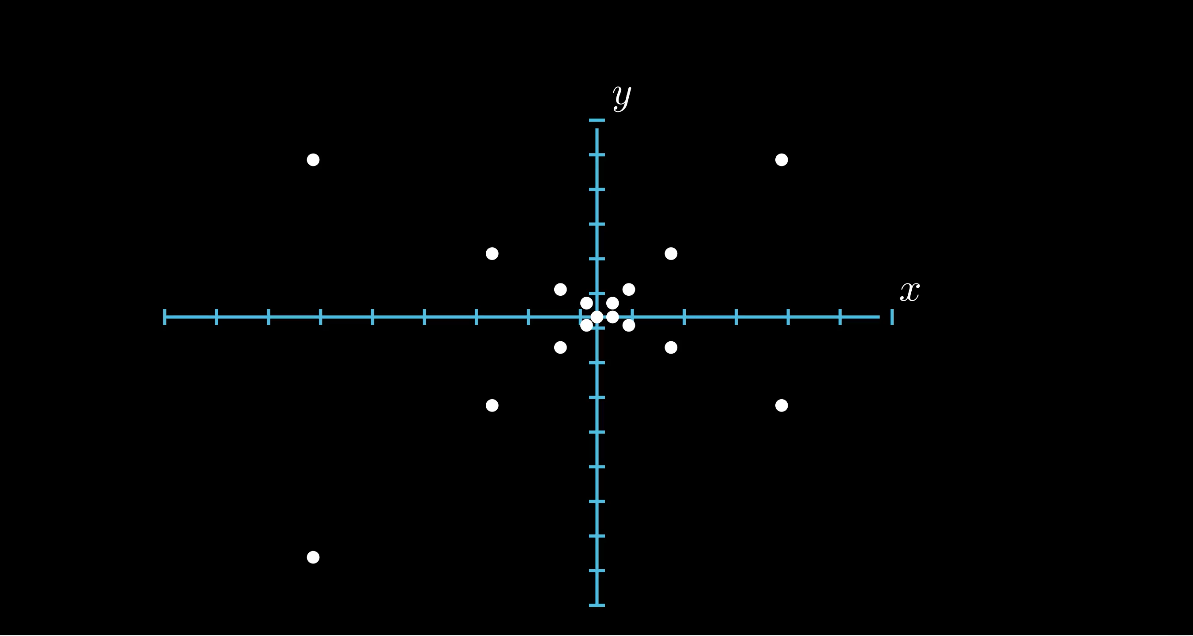
\includegraphics[scale=0.23, trim={3cm 0 6cm 0}, clip]{images/GFKT3.png}
		\caption{Plot of $P(n)$}
	\end{minipage}\hfill
	\begin{minipage}{0.45\textwidth}
		\centering
		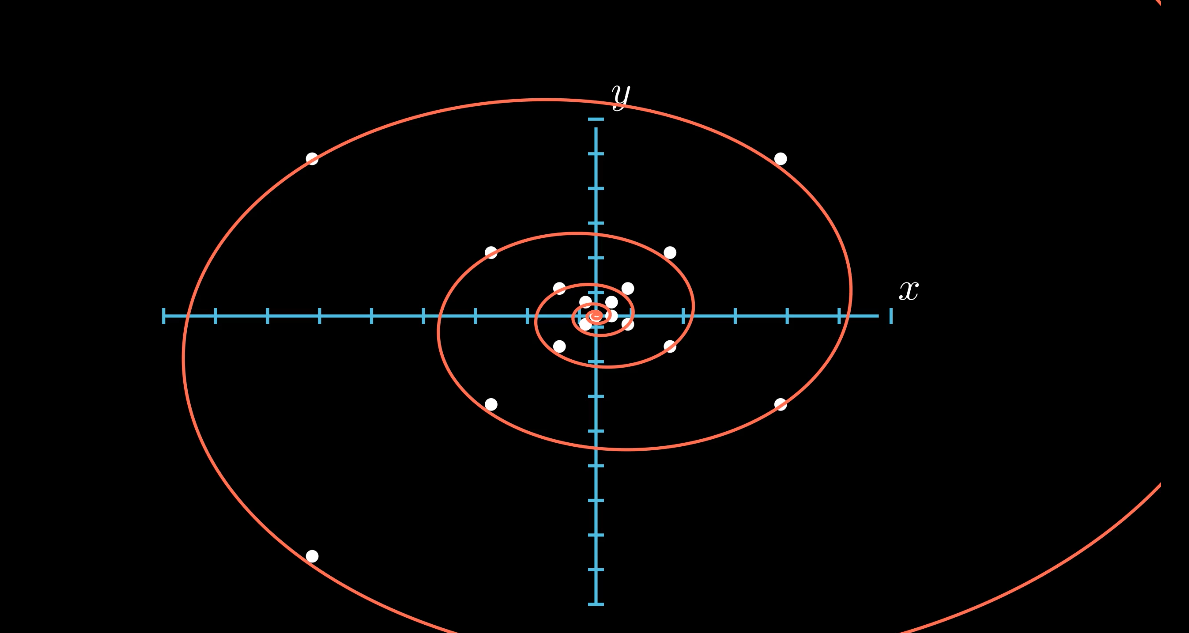
\includegraphics[scale=0.23, trim={3cm 0 6cm 0}, clip]{images/GFKT4.png}
		\caption{Logarithmic Spiral}
	\end{minipage}
\end{figure}
\begin{figure}[t]
	\label{figss}
	\centering
	\begin{minipage}{0.45\textwidth}
		\centering
		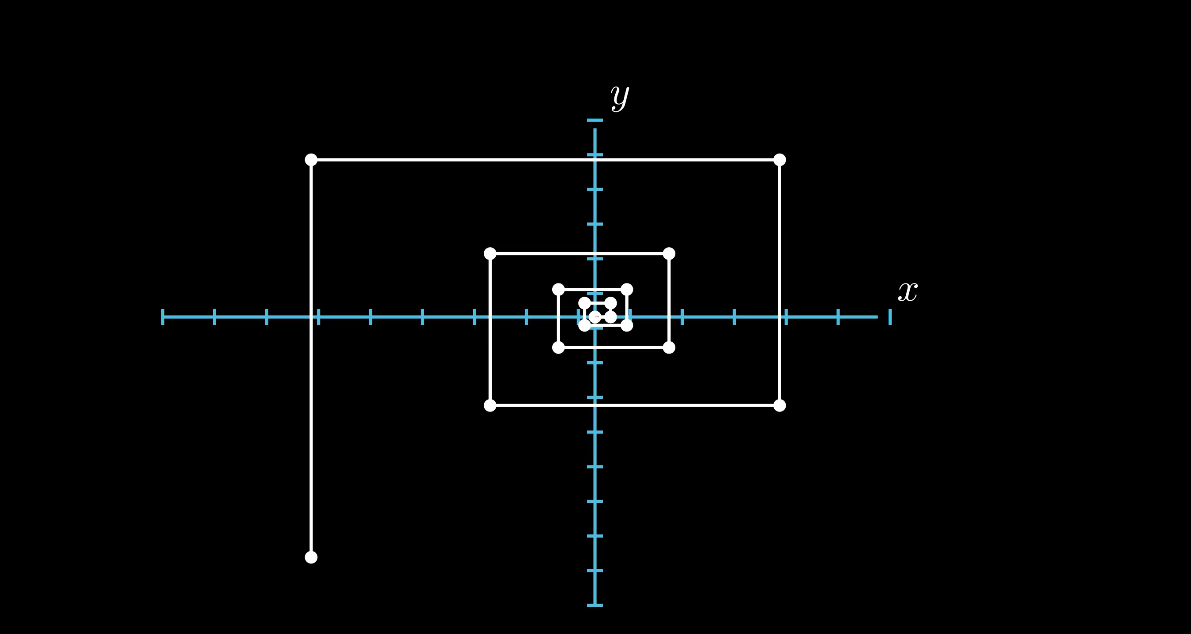
\includegraphics[scale=0.23, trim={3cm 0 6cm 0}, clip]{images/GFKT5.png}
		\caption{Plot of $L'(n)$}
	\end{minipage}\hfill
	\begin{minipage}{0.45\textwidth}
		\centering
		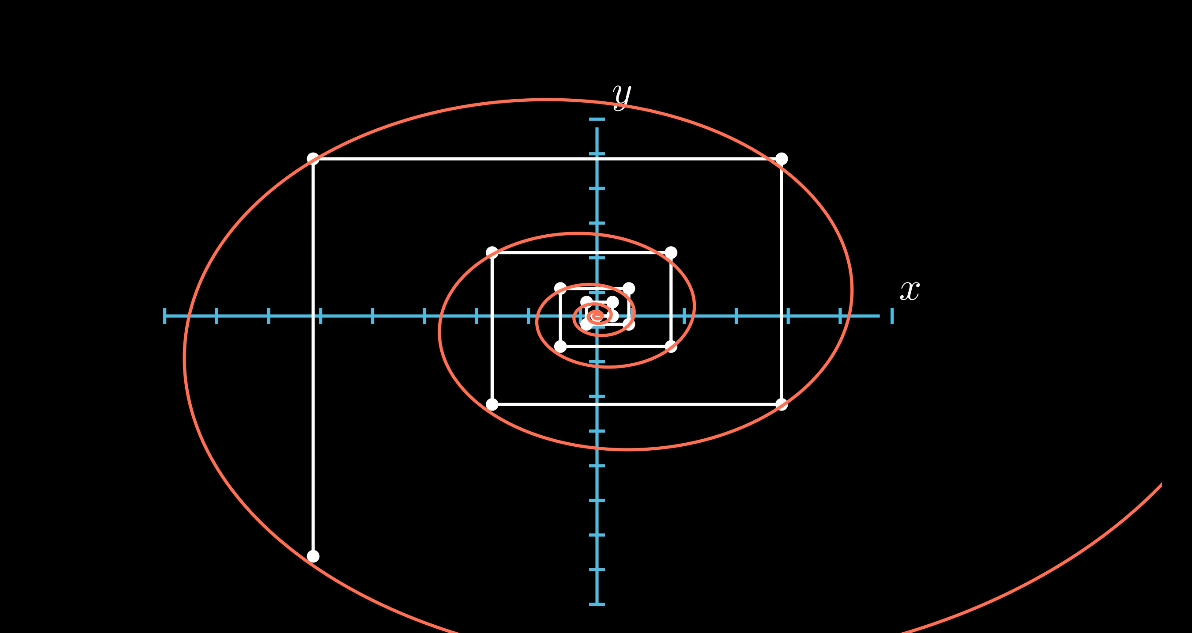
\includegraphics[scale=0.23, trim={3cm 0 6cm 0}, clip]{images/GFKT6.png}
		\caption{$L'(n)$ as discrete form of  logarithmic spiral}
	\end{minipage}
\end{figure}
\begin{figure}[t]
	\centering
	\begin{minipage}{0.45\textwidth}
		\centering
		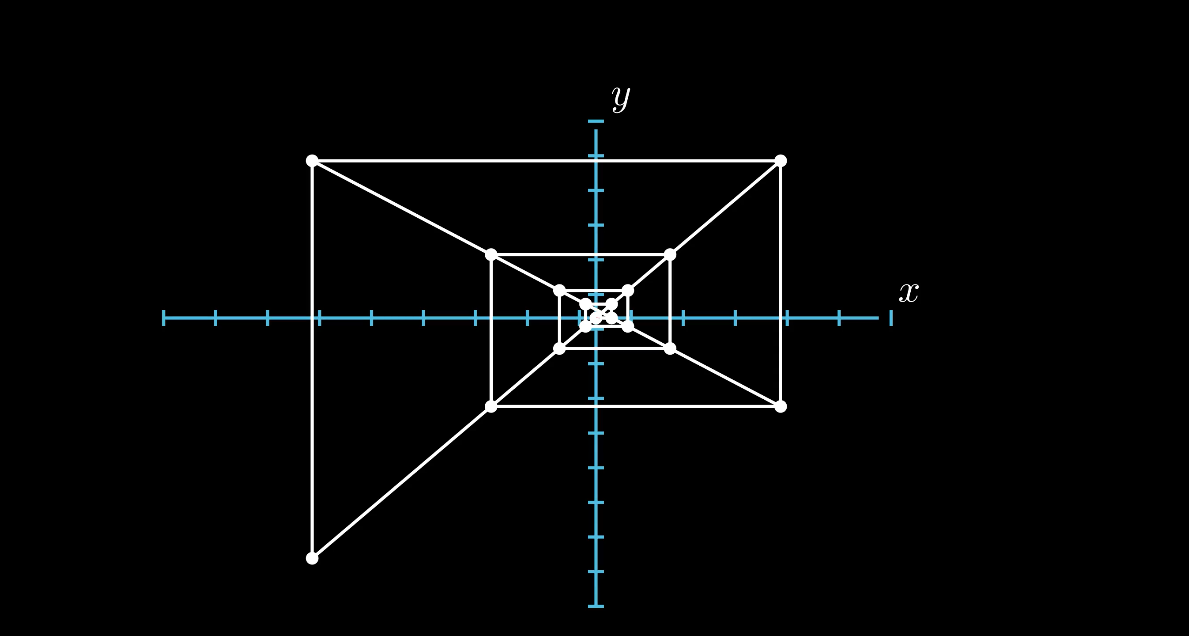
\includegraphics[scale=0.23, trim={3cm 0 6cm 0}, clip]{images/GFKT7.png}
		\caption{Plot of $T(n)$}
	\end{minipage}\hfill
	\begin{minipage}{0.45\textwidth}
		\centering
		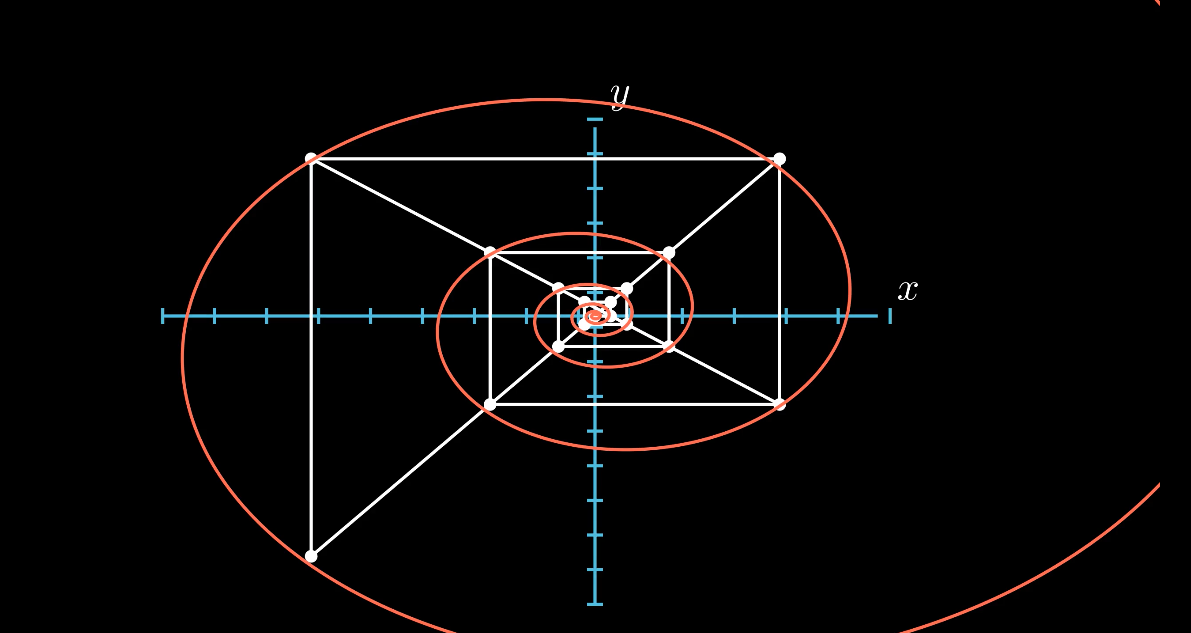
\includegraphics[scale=0.23, trim={3cm 0 6cm 0}, clip]{images/GFKT8.png}
		\caption{Complete Plot}
	\end{minipage}
\end{figure}

\section{Conclusion, Remarks and Extras}
We generalized a formula for recurrence relations that can be expressed as a linear combination of fibonacci numbers. Note that their limit can be modified under certain condition, let's make use of the fact that $\varphi^n = \varphi^{n-1}+\varphi^{n-2}$ \cite{PowerP}.\\
\begin{align*}
\begin{bmatrix}\varphi^n \\\varphi^{n-1}\end{bmatrix}
&=
\begin{bmatrix}1 & 1\\1 & 0\end{bmatrix}
\begin{bmatrix}\varphi^{n-1}\\\varphi^{n-2}\end{bmatrix}\\
\text{Therefore,}\\
\begin{bmatrix}\varphi^n \\\varphi^{n-1}\end{bmatrix}
&=
\begin{bmatrix}f'(n) & f'(n-1)\\f'(n-1) & f'(n-2)\end{bmatrix}
\begin{bmatrix}\varphi\\1\end{bmatrix}
\end{align*}
$\varphi^n = f'(n)\varphi+f'(n-1)$, recall from theorem \ref{lim-cons}, $c_{p',q'} = \dfrac{\varphi f_{a,b}(b+m_{p'})^a + f_{a,b}(m_{p'})^a}{\varphi f_{a,b}(b+m_{q'})^a + f_{a,b}(m_{q'})^a}$,\\\\
if the initial conditions are set such that $f_{a,b}(b+m_{p'})^a =f'(b+m_{p'}), f_{a,b}(m_{p'})^a = f'(b+m_{p'} -1)$ then, $c_{p',q'} = \varphi^{m_{p'}-m_{q'}}$ and $\displaystyle\lim_{n \to \infty} \dfrac{f_{a,b}(n + p)}{f_{a,b}(n + q)} = \left(\varphi^{d_{p',q'}+m_{p'}-m_{q'}}\right)^{1/a}$\\
To prevent the initial triangles from being skewed, the initial numbers should at least be within the same order of magnitude. Although all conditions still hold, the initial triangles appear a bit skewed if that is not the case.\\
We also convey that the functions $f_{a,1}$, produce a logarithmic spiral with equation, $$r = t\varphi^{2\theta/a\pi}$$ where $t=\left(\dfrac{\varphi f_{a,1}(1)^a+f_{a,1}(0)^a}{\varphi^{3}\sqrt{5}}\right)^{1/a}\varrho_{a,1}\sqrt{1 + \varphi^{2/a}}\hspace{2mm}\varphi^{-\left(\dfrac{ 2\tan^{-1}{\left(\varphi^{1/a}\right)}}{a\pi}\right)}$\\
So, we get logarithmic spirals whose growth factor is similar to $\varphi^{4/a}$, of course factoring in the constant $t$. The logarithmic spiral is found in nature at numerous places, due to its property of self-similar structure. Such as but not limited to spiral galaxies\cite{paper5}, spiral beaches\cite{paper6}.
\section*{References}
\begin{thebibliography}{9}
	\bibitem{paper1} 
	G. Anatriello, G. Vincenzi,
	Logarithmic spirals and continue triangles,
	Journal of Computational and Applied Mathematics,
	Volume 296,
	2016,
	Pages 127-137,
	ISSN 0377-0427,
	\doi{10.1016/j.cam.2015.09.004}
	URL\url{http://www.sciencedirect.com/science/article/pii/S0377042715004562}
	
	\bibitem{paper2}
	A. Fiorenza, G. Vincenzi, (2011), Limit of ratio of consecutive terms for general order- k linear homogeneous recurrences with constant coefficients. Chaos Solitons and Fractals - CHAOS SOLITON FRACTAL. 44. 145-152. \doi{10.1016/j.chaos.2011.01.003}
	
	\bibitem{paper3}
	L. Mario (2002). \href{https://archive.org/details/goldenratiostory00livi/page/149}{The Golden Ratio: The Story of Phi, The World's Most Astonishing Number.} New York: Broadway Books. p. 149. ISBN 0-7679-0815-5.
	
	\bibitem{paper4}
	P. Hemenway (2005). Divine Proportion: Phi in Art, Nature, and Science. Sterling Publishing Co. \href{https://en.wikipedia.org/wiki/Special:BookSources/978-1-4027-3522-6}{ISBN 978-1-4027-3522-6.}
	
	\bibitem{paper5}
	G. Bertin and C. C. Lin (1996). \href{https://books.google.com/books?id=06yfwrdpTk4C&pg=PA78}{Spiral structure in galaxies: a density wave theory.} MIT Press. p. 78. \href{https://en.wikipedia.org/wiki/Special:BookSources/978-0-262-02396-2}{ISBN 978-0-262-02396-2.}
	
	\bibitem{paper6}
	 A. T. Williams, A. Micallef (2009). \href{https://books.google.com/books?id=z_vKEMeJXKYC&pg=PA14}{Beach management: principles and practice.} Earthscan. p. 14. ISBN 978-1-84407-435-8.
	\bibitem{software}
	R. Gohil, (2020), \href{https://github.com/rahul-gohil/GFKT}{rahul-gohil/GFKT: GFKT@1.0.4} \doi{10.5281/zenodo.3784306}
	
	\bibitem{PowerP}
	G. Meisner, Powers of Phi, \href{https://www.goldennumber.net/powers-of-phi/}{https://www.goldennumber.net/powers-of-phi/}
\end{thebibliography}

\end{document}
